%-----------------------------------------------------------------------------
%
%               Template for sigplanconf LaTeX Class
%
% Name:         sigplanconf-template.tex
%
% Purpose:      A template for sigplanconf.cls, which is a LaTeX 2e class
%               file for SIGPLAN conference proceedings.
%
% Author:       Paul C. Anagnostopoulos
%               Windfall Software
%               978 371-2316
%               paul@windfall.com
%
% Created:      15 February 2005
%
%-----------------------------------------------------------------------------


\documentclass[preprint]{sigplanconf}


% The following \documentclass options may be useful:
%
% 10pt          To set in 10-point type instead of 9-point.
% 11pt          To set in 11-point type instead of 9-point.
% authoryear    To obtain author/year citation style instead of numeric.

\usepackage{amsmath}
\usepackage{amssymb}
\usepackage{listings}
\usepackage[pdftex]{graphicx}
\usepackage{verbatim} % only for comment environment
\usepackage{ifthen}

\graphicspath{{figures/}}
\DeclareGraphicsExtensions{.pdf, .png, .ps}   % NOT .jpg  because it throws away the detail.

\newboolean{showcomments}
\setboolean{showcomments}{true}
\ifthenelse{\boolean{showcomments}}
  {\newcommand{\nb}[2]{
    \fbox{\bfseries\sffamily\scriptsize#1}
    {\sf\small$\blacktriangleright$\textit{#2}$\blacktriangleleft$}
    % \marginpar{\fbox{\bfseries\sffamily#1}}
   }
  }
  {\newcommand{\nb}[2]{}
  }
\newcommand\apb[1]{\nb{apb}{#1}}
\newcommand\spj[1]{\nb{spj}{#1}}
\newcommand\je[1]{\nb{jeff}{#1}}

\begin{document}

\lstset{language=Haskell, basicstyle=\footnotesize, numbers=none, numberstyle=\footnotesize, stepnumber=1, numbersep=5pt, showspaces=false, showtabs=false, frame=none, tabsize=2, captionpos=b, breaklines=true, breakatwhitespace=false, xleftmargin=10pt,showstringspaces=false}
% ,resetmargins=true,breakindent=1cm,breakautoindent=true

% from http://www.haskell.org/haskellwiki/Literate_programming
\lstnewenvironment{code}
    {\lstset{}%
      \csname lst@SetFirstLabel\endcsname}
    {\csname lst@SaveFirstLabel\endcsname}
    \lstset{
      basicstyle=\small\ttfamily,
      flexiblecolumns=false,
      basewidth={0.5em,0.45em},
      literate={+}{{$+$}}1 {/}{{$/$}}1 {*}{{$*$}}1 {=}{{$=$}}1
               {>}{{$>$}}1 {<}{{$<$}}1 {\\}{{$\lambda$}}1
               {\\\\}{{\char`\\\char`\\}}1
               {->}{{$\rightarrow$}}2 {>=}{{$\geq$}}2 {<-}{{$\leftarrow$}}2
               {<=}{{$\leq$}}2 {=>}{{$\Rightarrow$}}2 
%               {\ .}{{$\circ$}}2 {\ .\ }{{$\circ$}}2
               {>>}{{>>}}2 {>>=}{{>>=}}2
               {|}{{$\mid$}}1               
    }

\conferenceinfo{ICFP 2011}{date, City.} 
\copyrightyear{2011} 
\copyrightdata{[to be supplied]} 

\titlebanner{Haskell for the cloud}        % These are ignored unless
\preprintfooter{Haskell for the cloud}   % 'preprint' option specified.


% \renewcommand{\floatpagefraction}{0.95}
% \renewcommand{\textfraction}{0.05}


%%%%% Andrew's commands
\newcommand{\ct}[1]{\textsf{#1}}

\newcommand{\nfn}{\ensuremath{\stackrel{\hash}{\rightarrow}}}
\newcommand{\nlambda}{\ensuremath{\lambda^\hash}\,}
\newcommand{\napp}{\ensuremath{\;\ct{\small \$}^{\hash}\,}}

\newcommand{\Int}{\mathbb{Z}}
\newcommand{\pair}[2]{\mbox{$\langle$#1, #2$\rangle$}}
\newcommand{\mpair}[2]{\mbox{$\langle #1, #2 \rangle$}}
\newcommand{\entails}{\vdash}
\newcommand{\hash}{\texttt{\#}}
\newcommand{\closed}[1]{\hash\,#1}
\newcommand{\textt}[1]{\lstinline!#1!}
\newcommand{\kmeans}{$k$-means}





\title{Haskell for the cloud}
\subtitle{}

\authorinfo{Jeff Epstein}
           {University of Cambridge}
           {jee36@cam.ac.uk}
\authorinfo{Andrew P. Black}
           {Portland State University\titlenote{Research conducted while on sabbatical at Microsoft Research, Cambridge.}}
           {black@cs.pdx.edu}
\authorinfo{Simon Peyton-Jones}
           {Microsoft Research, Cambridge}
           {simonpj@microsoft.com}

\maketitle

\begin{abstract}
% 1. What's the problem?
% 2. What does it matter?
% 3. What's the solution?
% 4. What are the consequences?
We present a framework for developing Haskell programs to be run in a distributed-memory computing environment. It provides a message-passing communication model, inspired by Erlang, without introducing incompatibility with Haskell's established shared-memory concurrency. We believe our framework will let Haskell programmers create fault-tolerant, high-performance distributed systems with a minimum of effort, while retaining Haskell's strengths in strong typing and shared-memory concurrent programming.

\end{abstract}

% \category{CR-number}{subcategory}{third-level}
\category{D.1.3}{Programming Techniques}{Concurrent Programming---Distributed Programming}
\category{D.3.2}{Programming Languages}{Haskell}
%\category{D.3.2}{Programming Languages}{Applicative (functional) languages}

\terms
Languages, Reliability, Performance

\keywords
keyword1, keyword2

\section{Introduction}

With the age of steadily improving processor performance behind us, the way forward is to compute with more, rather than faster, processors. A data center that makes available a large number of processors for storing and processing users' data, or running users' programs, is termed a \emph{cloud}. We'll use this term to mean specifically a network of computers that have independent failure modes and separate memories.

How should we program the cloud?  One approach is to simulate a familiar shared-memory multiprocessor, and then to program the simulated computer using conventional shared-memory concurrency primitives, such as locks and transactions. 
We have two objections to this approach.  The first is that the preponderance of the evidence is that shared-memory concurrency is \emph{just too hard}.  
\spj{Not a strong argument.  Message passing is always availble for shared memory machines and people don't use it much.  It's just
too inconvenient, or its cost model doesn't fit.  I'd nuke this objection.}
For example, 
$<<$Automatically classifying benign and harmful data races using replay analysis?$>>$
The second objection is that, to be effective, a programming model must be accompanied by a cost model: it must give programmers tools for reasoning about the cost of computation.  In a distributed memory system, one of the most significant costs is data movement; this is true whether one measures cost in terms of energy or time.  A programmer trying to reduce these costs needs a model in which they are explicit, not one that denies that data movement is even taking place\,---\,which is exactly the premise of a simulated shared memory. \spj{Not just data movement, but
cost of synchronisation too.  Eg distributed STM would be a disaster.}

Instead, we turn to a solution, popularized by MPI \cite{mpi99} and Erlang \cite{Erlang93}: {\em message passing}. The message passing model stipulates that the concurrent processes have no access to each other's data: any data that needs to be communicated from one process to another is explicitly copied by sending and receiving {\em messages}.  Not only does this make the costs of communication apparent; it also eliminates many of the classic concurrency pitfalls, such as race conditions. \spj{Again, I'd drop the race condition argument, and substitute the 
good failure model supported by message passing.}

Developing for the cloud presents other challenges.  In a network of dozens or hundreds of computers, some of them are likely to fail during the course of an extended computation; a programming system for the cloud must therefore be able to tolerate partial failure.  Here again, Erlang is has a solution that has stood the test of time; the highest reliability programs on the planet are written in Erlang, and achieve 9 nines reliability.  We don't innovate in this area, but adopt Erlang's solution (summarized in Section \ref{FaultTolerance}).

If Erlang has been so successful, you may wonder what Haskell brings to the table. 
The short answer is: purity, types, and monads.  As a pure functional language, data is by default immutable, so the lack of shared, mutable data won't be missed.  More importantly, the implementation can decide whether to share or copy immutable data: the choice is semantically invisible. Another consequence of purity is that functions are idempotent; this means that code running on failing hardware can be restarted elsewhere without the need for distributed transactions or other mechanisms for ``undoing'' effects.  
Types in general, and  type in particular, help to guarantee properties of programs statically.  
For example, a pure function \emph{cannot} have the same type as one that has an externally-visible effect such as sending or receiving a message.  
Monadic types make it convenient to program in an effectful style when that is appropriate, while ensuring that the programmer cannot accidentally mix up the pure and effectful code.

The contributions of this paper are:
\begin{itemize}
\item An interface for distributed programming in Haskell (Section \ref{Processes}). Following the Erlang model, our framework provides a system for exchanging messages between concurrent processes, regardless of whether those threads are running on one computer or on many. Besides mechanisms for sending and receiving data, we provide functions for starting new threads remotely, and for fault tolerance, which closely follow the widely-respected Erlang model. Unlike Erlang, our framework supports the use of explicit shared-memory concurrency mechanisms \emph{within} one of our concurrent processes.

\item A method for serializing function closures to enable higher-order functions to work in a distributed environment (Section \ref{Closures}). Starting a remote process demands a representation of code objects and their environment. Our approach to closures requires a \emph{explicit} indication of which parts of the function's environment will be serialized, and thus gives the programmer control over the cost of data movement.

\item A demonstration of the effectiveness of our approach in the form of example applications (Section \ref{Benchmarks}). We provide performance measurements from the $k$-means clustering algorithm, an iterative algorithm for partitioning data points into natural groups. The highly parallel nature of this algorithm makes it well-suited for deployment in a distributed environment.
\end{itemize}

\section{Processes and messages}
\label{Processes}
\subsection{Processes}
The basic unit of concurrency in our framework is the {\em process}. A process is a concurrent activity that has been ``blessed'' with the ability to send and receive messages. As in Erlang, processes are lightweight, with low creation and scheduling overhead.  Processes are identified by a unique process identifier, which can be used to send messages to the new process.

\begin{figure}
\centerline {
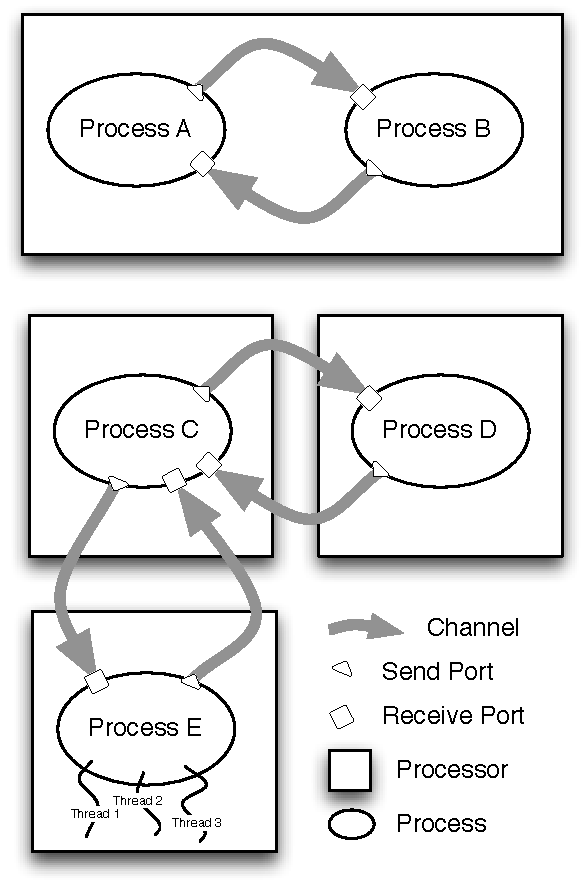
\includegraphics[width=\columnwidth]{threadsAndProcesses}
}
\caption{ \label{fig:ProcessBubbles}
Processes A and B do not share memory, even though they are running on the same physical processor; instead they communicate over channels, shown by grey arrows.  This makes it easy to reconfigure the application to resemble the situation shown with processes C and D.  Process E has created some lightweight threads using Concurrent Haskell's \texttt{forkIO} primitive; these threads share memory with Process E and with each other.  However, they cannot send or receive messages from Process E's channels, because this requires execution in the \texttt{ProcessM} monad; threads, in contrast, execute in the \texttt{IO} monad.
}
\end{figure}

In most respects, our framework follows Erlang by favoring message-passing as the primary means of communication between processes. Our framework differs from Erlang, though, in that it also supports shared-memory concurrency within a signle process. The existing elements of Concurrent Haskell, such as \textt{MVar} for shared mutable variables and \textt{forkIO} for creating lightweight threads, are still available to programmers who wish to combine message passing with the more traditional approach. This is illustrated in Figure \ref{fig:ProcessBubbles}. Our framework ensures that mechanisms specific to shared memory concurrency cannot be inadvertently used between remote systems.  \spj{Explain how!! This is very far from obvious and it's a key advantage.}

\subsection{Messages to processes}

Any process can send and receive messages. Our messages are asynchronous, reliable, and buffered.  All the state associated with messaging (most especially, the message queue) is wrapped in the \textt{ProcessM} monad, which is updated with each messaging action. Thus, any code participating in messaging must be in the \textt{ProcessM} monad.  The basic primitives are \textt{send} and \textt{expect}:

\spj{Add a note (foot?) to explain why expect not receive.}
\par{\small
\begin{code}
send :: (Serializable a) => ProcessId -> a -> ProcessM ()
expect :: (Serializable a) => ProcessM a
\end{code}}
(These type signatures, and those of all of the functions mentioned in this paper, are collected in Figure~\ref{fig:api}.)

Before we discuss these primitives in detail, let's look at an example of their use.
\textt{ping} is a process that accepts ``pong'' messages and responds by sending a ``ping'' to whatever process sent the pong. Using \textt{send} and \textt{expect}, the code for such a process would look like this:

\begin{code}
data Ping = Ping ProcessId
data Pong = Pong ProcessId
-- omitted: Serializable instance for Ping and Pong

ping :: ProcessM ()
ping = do { self <- getSelfPid
          ; Pong partner <- expect
          ; send partner (Ping self)
          ; ping }
\end{code}

\noindent The equivalent code in Erlang looks like this:

\begin{lstlisting}[language=Erlang]
ping() -> receive
           {pong, Partner} -> 
              Partner ! {ping, self()}
          end,
          ping().               
\end{lstlisting}

These two programs have similar structure. Both \textt{ping} functions are designed to be run as processes. They each wait for a specific message to be received; the Haskell \textt{expect} function matches incoming messages by type, whereas in Erlang, messages usually pattern-matched against tuples whose first element is a well-known atom. The programs wait for a ``pong'' message, and ignore all others. The ``pong'' message contains in its payload the process ID of a ``partner'', to whom the response message is sent; this message contains the process ID of the \textt{ping} process (\textt{self}). Finally, they wait for the next message by repeating with tail recursion.

If this example looks familiar, it should: it's very close to the first distributed programming example given in {\em Getting Started with Erlang}. Note that in the Haskell version, unlike in the Erlang version, \textt{Ping} and \textt{Pong} are types rather than atoms, and so they need to be declared explicitly. As given, the type declarations are incomplete; they need to be declared to be instances of the class \textt{Serializable}; we will discuss this in Section~\ref{s:serialization}.

In general, to send a message we use \textt{send}, which packages up an chunk of (serializable) data and transmits it (possibly over the network) to a particular process, given by its unique \textt{ProcessId}. Upon receipt, the incoming message will be placed in a message queue associated with the destination process. 
The \textt{send} function corresponds to Erlang's \texttt{!} operator.

\subsection{Serialization} \label{s:serialization}

\spj{Check for consistent spelling of serialize/serialize}
\spj{Somewhere we need to talk about Binary, and the relation of encode/decode to get/put.}

When we say that the data to be transmitted must be serializable, we mean that it must implement the \textt{Serializable} type class.  This ensures two properties: that the data is \textt{Binary} and \textt{Typeable} (see Figure~\ref{fig:api}).
\textt{Binary} means that \textt{put} and \textt{get} functions are available to encode and decode the data in binary form; \textt{Typeable} means a function \textt{typeOf} can be used to produce a representation of the data's type.  

While all of Haskell's primitive data types and most of the common higher-level data structures are instances of \textt{Serializable}, and therefore can be part of a message, some data types are emphatically not serializable. One example is \textt{MVar}, the type of Haskell's mutable concurrent variables. Since \textt{MVar} allows communication between threads on the assumption of shared memory, it isn't helpful to send it to a remote process that may not share memory with the current process. Although one can imagine a synchronous distributed variable that mimics the semantics of an \textt{MVar}, such a variable would have a vastly different cost model from a normal \textt{MVar}. Since neither \textt{MVar}'s cost model nor its implementation could be preserved in an environment requiring communication between remote systems, we felt it best to prohibit programmers from trying to use \textt{MVar}s in that way.  Notice, however, that we do not attempt to stop the programmer from using \textt{MVar}s within a single process: processes are allowed to use Haskell's \textt{forkIO} function to create \emph{local} threads that can share memory using \textt{MVar}.

\spj{What about receive?  Point out that parsing can fail, which makes use block, yes?}

At the far end of the channel, the simplest way of receiving a message is with \textt{expect}, which
examines the message queue associated with the current process and extracts the first message whose type matches the (inferred) type of \textt{expect}\,---\,a \textt{Ping} message in the example.  
\textt{expect} deques the message, unpacks the transmitted data and returns it.

%Together, they correspond to Erlang's \textt{receive} construct. Since our framework is packaged as a library rather than as a language extension, we use the \textt{MatchM} type to approximate Erlang's specialized syntax. \textt{receiveWait}'s first parameter is a list of \textt{match} invocations, where the lambda function argument to each \textt{match} potentially accepts a different type of message. Thus, the programmer can selectively dequeue messages of particular types. As in Erlang, incoming messages are tested in the order that the matching patterns appear. If no message in the queue is of any of the acceptable types, \textt{receiveWait} will block until such a message is received. % maybe mention matchIf, receiveTimeout, etc


%In the ping example above, we use \textt{receiveWait} and \textt{match} to accept messages only of type \textt{Pong}. The type of message to accept is specified through Haskell's type inference: the lambda function given as the first parameter to \textt{match} has type \lstinline!Pong -> ProcessM ()!, and so that invocation of \textt{match} will accept messages only of type \textt{Pong}.

\subsection{Starting processes}
\spj{This whole section needs a rewrite, and probably dramatically shortenig, in the light the closures section}

%\setlength{\parindent}{-3in}
\begin{figure}[t!]
\small
\textbf{Basic messaging} 
\begin{code}
send   :: Serializable a => ProcessId -> a
       -> ProcessM ()
expect :: Serializable a => ProcessM a
\end{code}
 \textbf{Channels}
\begin{code}
newChan  :: Serializable a 
         => ProcessM (SendPort a, ReceivePort a)
sendChan :: Serializable a 
         => SendPort a -> a -> ProcessM ()
receiveChan :: Serializable a => ReceivePort a
            -> ProcessM a
mergePortsBiased :: Serializable a => [ReceivePort a]
                 -> ProcessM (ReceivePort a)
mergePortsRR :: Serializable a => [ReceivePort a] 
             -> ProcessM (ReceivePort a)
\end{code}

 \textbf{Advanced messaging}
\begin{code}
receiveWait    :: [MatchM q ()] -> ProcessM q
receiveTimeout :: Int -> [MatchM q ()] 
               -> ProcessM (Maybe q)
match   :: Serializable a => (a -> ProcessM q) 
        -> MatchM q ()
matchIf :: Serializable a => (a -> Bool) 
        -> (a -> ProcessM q) -> MatchM q ()
matchUnknown :: ProcessM q -> MatchM q ()
\end{code}

 \textbf{Process management}
\begin{code}
spawn :: NodeId -> Closure (ProcessM ()) 
      -> ProcessM ProcessId
% call :: (Serializable a) => NodeId -> Closure (ProcessM a) -> ProcessM a
terminate :: ProcessM a
getSelfPid :: ProcessM ProcessId
getSelfNode :: ProcessM NodeId
\end{code}

 \textbf{Process monitoring}
\begin{code}
linkProcess :: ProcessId -> ProcessM ()
monitorProcess :: ProcessId -> ProcessId 
               -> MonitorAction -> ProcessM ()
\end{code}

 \textbf{Initialization}
\begin{code}
type RemoteTable = [(String,Dynamic)]
runRemote      :: Maybe FilePath -> [RemoteTable] 
               -> (String -> ProcessM ()) -> IO ()

type PeerInfo = Map String [NodeId]
getPeers       :: ProcessM PeerInfo
findPeerByRole :: PeerInfo -> String -> [NodeId]
\end{code}

 \textbf{Syntactic sugar}
\begin{code}
mkClosure     :: Name   -> Q Exp
remotable :: [Name] -> Q [Dec]
\end{code}

 \textbf{Logging}
\begin{code}
say :: String -> ProcessM ()
\end{code}

 \textbf{Type classes}
\begin{code}
class (Binary a,Typeable a) => Serializable a
class Typeable a where typeOf :: a -> TypeRep
class Binary t where { put :: t -> PutM (); get :: Get t }
encode :: Binary a => a -> ByteString
  -- Defined in terms of put
decode :: Binary a => ByteString -> a
  -- Defined in terms of get
\end{code}
\caption{A summary of the API.} \label{fig:api}
\end{figure}


To start a new process in a distributed system, we need a way of specifying where a process will run. The question of {\em where} is answered with our framework's unit of location, the node. A node can be thought of as an independent address space. Each node has a unique identifier, which contains the address and port number of a computer in the network. So, to be able to start processes, we want a function named \textt{spawn} that takes two parameters: a node identifier, saying on which computer the new process should run; and some expression of what code should be run there. Since we want to run code that is able to receive messages, the code should be in the \textt{ProcessM} monad. The function should then return a process identifier, which can be used with \textt{send}. And since the \textt{spawn} function itself depends on messaging, it, too, will be in the \textt{ProcessM} monad. As a first draft, let's consider this (incorrect) possibility:

\begin{code}
-- wrong
spawn :: NodeId -> ProcessM () -> ProcessM ProcessId
\end{code}

In combination with the \textt{ping} and \textt{pong} functions, it could be used like this:

\begin{code}
-- wrong
do { pingProc <- spawn someNode ping
   ; pongProc <- spawn otherNode pong
   ; send pingProc (Pong pongProc) }
\end{code}

The above example is supposed to start two new processes on \textt{someNode} and \textt{otherNode}, with each process expecting to receive messages of a particular type. To begin the exchange, we send an initial message to the ping process.

To understand why this version of \textt{spawn} is wrong, consider how to implement it. Assuming we have the ability to send messages containing arbitrary serializable data, \textt{spawn} can be implemented using \textt{send}.  \textt{spawn} will send a message containing its second parameter to a ``spawning'' process on the remote node; that is, a process that starts new processes in response to messages received from \textt{spawn}. In the above case, the call to \textt{spawn} would send a message containing the function \textt{ping}. And there's the sticky wicket. We can easily imagine how to serialize a string, or a list, or an algebraic data type composed of primitive types, but \textt{ping} is none of these. It's a function. And what does it mean to serialize a function? The question is especially important in a language like Haskell, where so much depends on higher-order functions manipulating other functions as data.

The other problem with serializing functions is that it isn't enough to serialize just the function: we also need its environment, precisely, its free names. Some of the free names used by the \textt{ping} function, such as \textt{receiveWait}, are top-level. Assuming that the same code is running on all hosts (a nontrivial assumption), it's not necessary to transmit the value of top-level names, as we know that they already exist at the destination node. But consider how to serialize a function that has free names that are not top-level, such as this one:

\begin{code}
-- wrong
printSumSomewhere :: NodeId -> Int -> ProcessM ()
printSumSomewhere aNode i =
  let nums = [0..i]
      fun = liftIO (putStrLn (show (sum nums)))
   in spawn aNode fun
\end{code}

This function accepts a location, given as a \textt{NodeId}, and an integer \textt{i}, and should remotely run the function \textt{fun}, which calculates the sum of integers $0 \ldots i$, and then prints out the result at the remote node. The list of integers $0 \ldots i$, named here \textt{nums}, is a free variable in \textt{fun}, but is not top-level. Furthermore, \textt{nums} depends on \textt{i}, which is also not top-level. Therefore, to be able to run \textt{fun} on a remote node, the local value of \textt{nums}, or at least \textt{i}, would need to be serialized and transmitted along with the representation of \textt{fun}.

There are a few reasons why we don't want to automatically transmit the whole of \textt{fun}'s environment. The first reason is that it's hard to do without extending the language. In order to discover what names need to be included as part of a serializable environment, we would need to traverse \textt{fun}'s abstract syntax tree, picking up free variables along the way, and in turn the transitive closures of their free variables, as well. Since our framework is implemented solely as a library, we'd prefer to avoid the compiler-hacking that would be necessary.

Another reason why implicit serialization of environment is bad is that it's easy for the programmer to lose track of what's being serialized. Since over-the-wire communication is potentially the greatest bottleneck in a distributed application, it's important that the programmer have direct control over what is transmitted. In the above code, for example, \textt{i} may be serialized, even though it isn't mentioned in \textt{fun}. To keep the quantity of serialized data under control, we prefer an explicit approach to environment serialization.

Finally, we should mention that in a non-strict language such as Haskell, implicit serialization of environment raises some thorny questions about what is evaluated and where. How, exactly, should \textt{fun}'s environment be serialized? One way would be for the value of \textt{nums} to be sent. Another way would be for the value of \textt{i} to be sent, along with a representation of \textt{nums} that depends on the value of \textt{i}. In the first option, depending on the size of \textt{nums}, a lot of data could potentially be transmitted. In the second option, there would probably be fewer bytes sent, at the cost of having to evaluate \textt{nums} remotely. There are several possible ways a language could balance these trade-offs, but the answer is likely to be somewhat arbitrary and not transparent to the programmer. This is another case where the programmer loses control of the cost model, and, again, we aimed for a more explicit interface.

In our framework, a captured environment is never transmitted implicitly. We accomplish this by restricting the set of serializable functions to those without non-top-level free variables. This is discussed further in section 3.

\subsection{Fault tolerance}
\label{FaultTolerance}
We aimed to follow as closely as possible Erlang's model for fault tolerance. Erlang's \textt{link} and \textt{monitor} functions allow processes to request notification if another process terminates. We provide analogous functions that offer similar functionality.

Our fault tolerance API is based on the idea that a process can monitor another process. If the monitored process terminates, the other process will be notified, and can take appropriate action. We provide relatively only low-level functions that allow for notification of possible faults. Actually recovering from faults is left to the application or a higher-level framework, such as the one briefly discussed in the Future work section.

A process can request to be notified in the event that another process terminates for any reason, or only in the case of a fault involving that process. A fault that will result in a notification can be caused either by the other process being terminated as a result of an uncaught exception, or if the node on which the process is running becomes inaccessible. The monitoring process can also indicate to be notified in one of two ways: either by an asynchronous exception, which can be caught with Haskell's usual exception handling mechanisms; or by message, which can be received using the \textt{receiveWait} function.

Here are the functions for setting up process monitoring:

\begin{code}
monitorProcess :: ProcessId -> ProcessId
               -> MonitorAction -> ProcessM ()
linkProcess    :: ProcessId -> ProcessM ()
\end{code}

\lstinline!monitorProcess a b ma! establishes unidirectional process monitoring. That is, process \textt{a} will be notified if process \textt{b} terminates. The third argument determines whether the monitoring process will be notified by exception or by message.

\textt{linkProcess} corresponds to Erlang's \textt{link}. It establishes bidirectional process monitoring between the current process and a given process; if either of those processes terminate abnormally, the other will receive an asynchronous exception. \textt{linkProcess} is defined in terms of \textt{monitorProcess}. 

\section{Matching messsages}

In the previous section, we introduced the \textt{expect} function, which lets us receive messages of a particular type. But what if our process wants to be able to accept messages of different types? Ideally, we'd like to be able to approximate the Erlang \textt{receive} syntax:
\begin{lstlisting}[numbers=left,language=Erlang,escapeinside={\%}{\^^M}]
math() ->
  receive
    {add, Pid, Num1, Num2} -> % \label{erl_addmatch}
      Pid ! Num1 + Num2; % \label{erl_addhandler}
    {divide, Pid, Num1, Num2} when Num2 /= 0 -> % \label{erl_divmatch}
      Pid ! Num1 / Num2;
    {divide, Pid, _, _} ->
      Pid ! div_by_zero
  end,
  math().
\end{lstlisting}

This code will accept and respond to several different messages. It does this by pattern matching on the values of the messages, expressed as tuples. Each pattern has a corresponding message-handling action. At line \ref{erl_addmatch}, it matches a tuple containing the atom \textt{add}, a process ID, and two numbers; when it receives a message matching that form, it will invoke the corresponding handler on line \ref{erl_addhandler}, which sends the sum of the two numbers. In the next pattern, on line \ref{erl_divmatch}, it responds similarly to a message with a \textt{divide} atom, but only if the divisor is not zero; this is controlled by the optional \textt{where} syntax. Finally, the third pattern will send a \textt{div_by_zero} atom in response to requests for division in those cases not matched by the previous patterns, which is to say, those cases when the divisor is zero. Patterns are tested against each message in the order that they appear, so that the last pattern will only be reached if the first two fail to match.

Haskell doesn't have an atom data type, but an idiomatic way of representing the different messages is to use Haskell's type system. For each distinct message, distinguished in Erlang by the first member of the tuple, we will have a separate type. Thus, we can imagine these types:

\begin{code}
data Add = Add ProcessId Double Double
data Divide = Divide ProcessId Double Double
data DivByZero = DivByZero
\end{code}

Clearly, \textt{expect} is not up to the task of translating the above code. \textt{expect} can accept only one of type of message, and will block until a message of that type is put in the message queue. In the interim, any other messages will simply accumulate in the message queue. How can we represent the branching structure of Erlang's \textt{receive} in Haskell?

First, let's consider how to specify to specify a pair consisting of a message type and its corresponding action. We introduce \textt{match}, which accepts as a parameter a function that maps a message to an action. \textt{match}'s job is to determine if a message in the queue has the appropriate type, and if so to invoke the user-provided function with the message as its argment.

\begin{code}
match :: (Serializable a) => (a -> ProcessM q) -> MatchM q ()
\end{code}

When \textt{match} tests an incoming message, it is comparing the type of the incoming message against the type \textt{a}. Any message of that type will be considered matched, and will be removed from the message queue, and the message handler will be invoked.

\textt{match} is in the \textt{MatchM} monad, which is responsible for providing \textt{match} with the current state of the message queue, and then providing \textt{match}'s caller with the result of its test. \textt{match} will typically be used with \textt{receiveWait}, which mimics Erlang's \textt{receive} syntax by evaluating several \textt{MatchM}'s in order. The value returned by the selected message action is also the return value of \textt{receiveWait}.

\begin{code}
receiveWait :: [MatchM q ()] -> ProcessM q
\end{code}

And how can we handle Erlang's \textt{where} clause, which allows message acceptance to be qualified by a predicate? We offer \textt{matchIf}, whose first parameter is allowed to examine the incoming message without removing it from the queue.

\begin{code}
matchIf :: Serializable a => (a -> Bool) -> (a -> ProcessM q) -> MatchM q ()
\end{code}

Below we implement the \textt{math} function in Haskell. Notice that the patterns from the Erlang version have been replaced with parameters to lambda functions.

\begin{code}
-- omitted: Serializable instances for Add, Divide, and DivByZero types
math :: ProcessM ()
math =
  receiveWait
    [ match   (\(Add pid num1 num2) -> 
                send pid (num1 + num2)),
      matchIf (\(Divide _ _ num2) -> num2 /= 0) 
              (\(Divide pid num1 num2) -> 
                send pid (num1 / num2)),
      match   (\(Divide pid _ _) -> 
                send pid DivByZero) ]
        >> math
\end{code}
%\)

The combination of \textt{receiveWait} and \textt{match} closely corresponds to Erlang's \textt{receive} syntax. The list of \textt{MatchM}s are tested in order against each message in the message queue. When a matching message is found, the corresponding lambda function is invoked. 
Matching by message type is not quite the same as matching by message value. For example, if a particular \textt{match} accepts message of a type, then all variants of that type must be handled. In the above example, this is okay, because the \textt{Add} type has only the \textt{Add} constructor. If there were another constructor, then the \textt{match} call that expects only the \textt{Add} constructor would cause a pattern match exception if a message with the other constructor were received.

Clearly, \textt{receiveWait} is more flexible than \textt{expect}. In fact, \textt{expect} is implemented in terms of \textt{receiveWait}. Its definition looks like this:

\begin{code}
expect :: (Serializable a) => ProcessM a
expect = receiveWait [match return]
\end{code}

\section{Messages through channels}
In the previous subsection, we've shown how a message can be sent to a process. As you can see from the type signature of \textt{send}, essentially any serializable data structure can be sent as a message to any process. Whether or not a particular message will be accepted (i.e. dequeued and acted upon) by the recipient process isn't determined until runtime. But what about Haskell's strong typing? Wouldn't it be nice to have some static guarantees that we are sending a message type to a receiver that knows how to deal with it?

Thus, an alternative to sending messages by process identifier is to use {\em typed channels}. Each distributed channel consists of two ends, which we call the {\em send port} and {\em receive port}. Messages are inserted via the send port, and extracted in FIFO order from the receive port. Unlike process identifiers, channels are associated with a particular type and the send port will emit messages only of that type; likewise, the receive port will accept messages only of that type, so the sender has a guarantee that its receiver is of the right type.

The central functions of the channel API are:
\par{\small
\begin{code}
newChan  :: Serializable a 
         => ProcessM (SendPort a, ReceivePort a)
sendChan :: Serializable a => SendPort a -> a -> ProcessM ()
receiveChan :: Serializable a => ReceivePort a -> ProcessM a
\end{code}}

A critical point is that although \textt{SendPort} can be serialized and copied to other nodes, allowing the channel to accept data from multiple sources, the \textt{ReceivePort} cannot be moved from the node on which it was created. We decided that allowing a movable and copyable message destination would introduce too much complexity. This restriction is enforced by making \textt{SendPort} an instance of \textt{Serializable}, but not \textt{ReceivePort}. 

We can now reformulate our ping example to use typed channels. The process must be given two ports: a receive port on which to receive pongs, and a send port on which to emit pings. Each \textt{Ping} and \textt{Pong} message now contains the send port on which its recipient should respond; thus the \textt{Ping} message contains the send port of a channel of pongs, and the \textt{Pong} message contains the send port of a channel of pings.

% this might not be the best example, really
\begin{code}
ping2 :: SendPort Ping -> ReceivePort Pong -> ProcessM ()
ping2 pingout pongin = 
   do { (Pong partner) <- receiveChan pongin
      ; sendChan partner (Ping pongin) 
      ; ping pingout pingin }
\end{code}

How do we start the exchange? Clearly we need to create two channels and call \textt{ping2} and \textt{pong2} (not shown, but substantially similar to \textt{ping2}) as new processes. But how do we start a new process?

\spj{Somwhere we need to say that send-ports are serializable and read-ports are not. It's a key property!
Indeed that is why we distinguish the end-points.}


\section{Closures}
\label{Closures}
\begin{comment}
there's no way for a library to know what to transmit, or even if it's serializable. Clearly, we don't want to prevent remotely-invocable functions from ever using non-serializable data. That would mean that any function that could be started using \textt{spawn} wouldn't be allowed to use \textt{MVar}.

all parameters to closure must be serializable

I agree that all we need to do to represent deferred evaluation is a
<fun,arg> tuple, and that's basically what a Closure is. We'll still
serialize arbitrarily-sized environments, as long as they are
converted explicitly to an argument, and that explicit control is an
advantage. And, yes, the practical argument that implicitly
serializing environments would be messy to implement is also valid.

only local and global names are visible in a top-level function. This is a reasonable approximation because all toplevel names are always available on all hosts and never need to be transmitted

prevention of sharing bad things (e.g. mvars, receiveports) is enforced by the serializer
\end{comment}
% ----------------------------------------------- BEGIN SIMON

Any distributed implementation of a statically-typed, 
higher-order programming language must
grapple with the fundamental question of \emph{how to transmit closures} from
one node to another.  For example, consider:
\begin{code}
  sf :: SendPort (Int -> Int) -> Int -> ProcessM ()
  sf p x = send p (\y -> x+y+1)
\end{code}
\texttt{sf} is a function that creates an anonymous function and sends it on Port\texttt{p}.   The function that it sends, \texttt{($\lambda$y -> x+y)},
is a closure that captures its free variables,
in this case \textt{x}; 
in general, to serialize a function value requires that one must also serialize its free variables.  But the types of
these free variables are unrelated to the type of the function
value, so it is entirely unclear \emph{how} to serialize them.
\apb{in a library that knows only the type of the function itself}.
In concrete terms, there is no way to write this instance
declaration
\begin{code}
  instance ???? => Serializable (a->b) where ????
\end{code}
One ``solution'' would be to say that functions are simply not
serializable --- but exactly the same issue arises with \textt{spawn}:
\begin{code}
newComputation = 
  do { (s,r) <- newChan
      ; spawn node (do { answer <- longComputation
                  	   ; sendChan s answer })
      ; receiveChan r}
\end{code}
The second argument of \textt{spawn}, the code that we want to run on the remote \textt{node}, is a value closed over
its free variables, \textt{s}.
Thus, serializing this argument requires serializing a function with a free variable.
We can't avoid this problem, because the essence of distributed computation is 
a way of start a remote computation; in a higher-order language like Haskell, that must inevitably
involve serializing a closure of some kind.

\subsection{The standard solution}

The standard approach to this problem is to bake in serialization of
function values --- and indeed of all values --- as a primitive operation
implemented directly by the runtime system.  That is, the runtime system
allows one to serialize \emph{any value at all}, and transport it to the 
other end of the wire.  Now function closures can be serialized by
serializing their free variables, and adding a representation of their code.
This approach is used by every higher-order distributed-memory 
system that we know of, including GDH \cite{gdh2001}, JoCaml (check!!!), \emph{what else}.

\apb{I don't think that this is true; I think that the standard solution is reflection.
This does not have the first two disadvantages that you list, but t does have the third.}
Making serializability built-in
has multiple disadvantages:
\begin{itemize}
\item It relies on a single built-in notion of serializability.
In contrast, the \texttt{Serializable} type class introduced in 
Section~\ref{s:serializable} gives the programmer control over how
values are serialized.  For example, a data structure might have
redundant information cached in the nodes, which should be reconstructed
at the far end rather than being serialized.  
This is exactly what type
classes are for!
\item It is crucial that some types are \emph{not} serializable. For
example, we do not want the receive port of a channels to be serializable, 
so that senders know where to send their messages to.  Similarly making 
\textt{TVar}s non-serializable guarantees that \textt{STM} transactions 
do not span processes.
\item Serializing a value and sending it over the network has an important
effect on the cost model; it should not be silent.
\end{itemize}
In short, built-in serializability of every value is
too big a primitive.  We do need \emph{some} built-in support, but
we seek something more more modest.  Proposing such a mechanism is one of 
the main contributions of this paper.

\subsection{Static values}

We begin with a simple intuituion: some closures can readily be
transmitted to the other end of the wire, namely ones that have no
free variables.  For the present we make a simplifying assumption,
that every node is running the same code.  (We return to the question
of code that varies between nodes in Section~\ref{s:code-update}.)
Under this assumption, a closure without free variables can be
readily be serialized to a single symbolic code address, also called a linker label.

To distinguish values that can be readily serialized from those that cannot, we introduce a new type constructor
$(\text{\tt Static}~\tau)$ to classify such values.  The type 
constructor \textt{Static} is a new built-in primitive, 
enjoying a built-in serialization instance:
\begin{code}
  instance Serializable (Static a)
\end{code}
It is helpful to remember this intuition: \emph{the defining property of
a value of type $(\text{\tt Static}\;\tau)$ is that it can be serialized},
moreover, that it can be serialized without knowledge of how to serialize $\tau$.
Operationally, the implementation serializes a \textt{Static} value by first evaluating it,
and then serializing the code label in the result of the evaluation.  

\begin{figure}[t!]
\begin{minipage}{\linewidth}
$$
\begin{array}{rcl}
\Gamma & ::= & \overline{x :_{\delta} \sigma} \\
     \delta & ::= & S | D
\end{array}
$$
\begin{align*}
\Gamma\downarrow = \{ x:_{s} \sigma \mid x :_{s} \sigma \in \Gamma \}
\end{align*}

\begin{equation*}
\tag{Static~intro.}
\frac{\Gamma\downarrow~\entails e : \tau}
     {\Gamma \entails \text{\tt static}~e : \text{\tt Static}~\tau}
\end{equation*}

\begin{equation*}
\tag{Static~elim.}
\frac{\Gamma \entails e : \text{\tt Static}~\tau}
     {\Gamma \entails \text{\tt unstatic}~e : \tau}
\end{equation*}
\end{minipage}
\caption{Typing rules for \textt{Static}} \label{fig:static}
\end{figure}
Along with the new type constructor we introduce a new term,
$(\text{\tt static}\;e)$ to introduce it, and another 
$(\text{\tt unstatic}\;e)$ to elimiate it.
The typing judgements for these terms are given in Figure~\ref{fig:static}.
They embody the following key ideas:
\begin{itemize}
\item A \emph{variable is static} iff it is bound at the top level.
\item A \emph{term $(\text{\tt static}\;e)$ has type $(\text{\tt Static}\;\tau)$} iff 
$e$ has type $\tau$, and $e$ is static.  
\end{itemize}
The type environment $\Gamma$ is a set of variable bindings, each of form $x :_{\delta} \sigma$.
The subscript $\delta$ is a static-ness flag, which takes the values \textt{S} (static) or
\textt{D} (dynamic).  The idea is that top-level (static) variables have bindings
of the form $f\! :_{\text{\tt S}}\! \sigma$, while all other variables have dynamic bindings 
$x\! :_{\text{\tt D}}\!\sigma$.
(It is straightforward to formalise this idea in the typing judgements for top-level
bindings and for terms; we omit the details.)
The operation $\Gamma \downarrow$ filters $\Gamma$ to leave only the
static (top-level) bindings,thereby checking that a term $\text{\tt
static}\;e$ is well typed only if all its free variables are static.

Although simple, these rules have interesting consequences:
\begin{itemize}
\item A static variable may have a non-\textt{Static} type. Consider the 
top-level binding for the identity function:
\begin{code}
  id :: a -> a
  id x = x
\end{code}
The function \textt{id} is by definition static (top-level).  Its binding
in $\Gamma$ will have $\delta=\text{\tt S}$, but its type is the ordinary
polymorphic type. However, \textt{(Static id)} has type \textt{(Static (a -> a))}.


\item A non-static variable may have a \textt{Static} type.  For example
\begin{code}
  f :: Static a -> (Static a, Int)
  f x = (x, 3)
\end{code}
Here \texttt{x} is lambda-bound and so is not a static variable, but it certainly has
a \textt{Static} type.  So fully-dynamic functions
can readily compute over values of \textt{Static} type.

\item The free variables of a term $(\text{\tt static}\;e)$ need not have
\text{\tt Static} types. For example, this term is well-typed:
\par{\small
\begin{code}
static (length . filter id) :: Static ([Bool] -> Int)
\end{code}
}
because all its free variables (\textt{length}, \textt{(.)},
\textt{filter}, \textt{id}) are bound at top-level and hence are
static. However, all these functions have their usual types.
\end{itemize}

\subsection{From static values to closures}

In the examples \textt{sf} and
\textt{nc} (at the start of this Section) we wanted to transmit closures
that certainly did have free variables.  How do static values help us?
They help us by making \emph{closure conversion} possible. A closure
is just a pair of a code pointer and an environment.  With the aid of
\textt{Static} values we can now represent a closure directly in Haskell:
\begin{code}
data Closure a where   -- Wrong
  MkClosure :: Static (e -> a) -> e -> Closure a
\end{code}
As is conventional, we capture the environment in an existential\footnote{
Existential because \textt{MkClosure}'s type is isomorphic 
to $\forall a. (\exists e. (e \to a) \times e) \to \text{\tt Closure}\;a$.
}.
\apb{More explanation needed.  Since there are no existential quantifiers here, this is hard to follow as written.  You have encoded the existential as an (unwritten) universal on the LHS of an arrow; this is not obvious!}
Different closures of the same type may thereby capture environments
of different type.  For example,
\begin{code}
  cs :: [Closure Int]
  cs = [MkClosure (static negate) 3,
        MkClosure (static ord)   'x']
\end{code}
Both closures in the list \textt{cs} have the same type \textt{Closure Int},
but the first captures an \textt{Int} as its environment, while the second
captures a \textt{Char}.  (The function \textt{ord} has type \textt{Char->Int}.)

The trouble is that this closure type is not serializable: precisely
because the environment is existentially quantified, there is no information
for how to serialize it!  This is apparently esay to solve, by asking
that the environment be serializable:
\begin{code}
data Closure a where   -- Still wrong
  MkClosure :: Serializable env
        => Static (env -> a) -> env -> Closure a
  deriving( Typeable )
\end{code}
Now serialization is easy:
\begin{code}
instance Binary (Closure a) where
   put (MkClosure f env) = put f >> put env
\end{code}
But how can we \emph{de}-serialize a closure?  The difficulty is
that, at the receiving end, we do not know the type captured inside
the closure, so we do not know what deserializer to use.  This initially
appears to be a very awkward problem indeed. Maybe we have to send a 
representation of the environment type, and do a run-time type-class lookup
at the receiving end?  This solution is used by Clean \cite{clean}.  Maybe
we could send some representation of the deserialization function itself?
But that seems to require a solution to the problem of serializing 
closures, so an infinite regress beckons.

Happily, the solution is simple and, with the benefit of hindsight,
obvious: perform both serialization and deserialization at \emph{closure-construction time},
not at \emph{closure-serialization time}:
\begin{code}
data Closure a where   -- Right
  MkClosure :: Serializable env
        => Static (ByteString -> a) 
        -> ByteString -> Closure a
\end{code}
Now the correct deserializer becomes part of the static code pointer 
in the closure.  Simple.

It is easy to un-closure-convert:
\begin{code}
  unClosure :: Closure a -> a
  unClosure (MkClosure f x) = unstatic f x
\end{code}
This is when the deserialization of the environment takes place. For a
function-valued closure it makes sense to apply \textt{unClosure} once, and
apply the resulting function many times, so that the deserialization is
one just once.

\subsection{Closures in practice} \label{s:closures-in-practice}

To see closures in action, here is our earlier \textt{sf} example, 
expressed using closures:
\begin{code}
  sf :: SendPort (Closure (Int -> Int)) 
     -> Int -> ProcessM ()
  sf ch x = send ch clo
    where
      clo  = MkClosure (static sfun) (encode x)

  sfun :: ByteString -> Int -> Int
  sfun = \bs -> let x = decode bs 
             in \y -> x + y + 1)
\end{code}
The closure contains the pre-serialized environment \textt{encode x},
and the static function \textt{sfun}. The latter deserializes its
argument \textt{bs} to get the real argument \textt{x} that it expects.

As a second example, consider \textt{nc} from the beginning of this section.
Using closures we would rewrite it like this:
\begin{code}
  nc :: ProcessM ()
  nc = do { (s,r) <- newChan
          ; spawn node (MkClosure (static child) (encode s))
          ; ... }

  child :: ByteString -> ProcessM ()
  child = \bs -> let s = decode bs
              in do { ...ans...
                    ; sendChan s ans })
\end{code}
The type of \texttt{spawn} is given in Figure~\ref{fig:api}; it takes
a closure as its second argument.

\subsection{Summary}

In this section we introduced a rather simple set of language primitives:
\begin{itemize}
\item A new type constructor \textt{Static}, with built-in serialization.
\item A new term form $(\text{\tt static}~e)$.
\item A new primitive function \textt{unstatic :: Static a -> a}.
\end{itemize}
Building on these primitives we can manually construct closures and
control exactly how and when they are serialized.
Performing manual closure conversion is tiresome for the programmer,
and one might wonder about adding some syntactic sugar.
We have not yet explored this option very much, preferring to work out the
foundations first.
However in the next section we describe some simple Template Haskell support.

% A more intrusive drawback of our approach is that serialization cannot
% handle existential data types or generalized abstract data types
% (GADTs) at all. That is, no remotely invoked function can accept an
% existential or GADT parameter or return such a type. The problem is
% that these extended Haskell types can hide constituent data types that
% are not reflected in the signature of the enclosing type. As a result,
% the type-based dispatch for serializing and deserializing them has no
% way to know which concrete serializer and deserializer to invoke. As
% far as we know, serializing existentials and GADTs would require some
% form of run-time introspection, and Haskell does not currently provide
% that.


\section{Faking it}

We have not yet implemented statics in GHC, but we have implemented
some simple workarounds that allow us (and you, gentle reader) to experiement
with them without changing GHC.  We describe these workarounds in this section.

\subsection{Example}
As a running example, here is the code for \textt{sfun} using the workarounds:
\begin{code}
  sf :: SendPort (Closure (Int -> Int)) 
     -> Int -> ProcessM ()
  sf ch x = send ch ($(mkClosure 'add1) x)

  add1 :: Int -> Int -> Int
  add1 x y = x + y + 1

  $(remotable ['add1])
\end{code}
The programmer still has to do manual closure conversion, by defining
a top-level function (\textt{add1} in this case) whose first argument is
the environment.  However, the code is otherwise significantly more 
straightforward than in Section~\ref{s:closures-in-practice}.

The Template Haskell splice \textt{$(mkClosure 'add1)}
is run at compile time.  Its argument \textt{'add1} is Template Haskell notation
for the (quoted) name of the \textt{add1} function.
\begin{code}
  mkClosure :: Name -> Q Exp
\end{code}
The splice expands to a call to \textt{add1__closure}, 
so the net result is just as if we had written
\begin{code}
  sf ch x = send ch (add1__closure x)
\end{code}
What is \textt{add1__closure}?  It is a new top-level definition
added by the Template Haskell splice \textt{$(remotable ['add1])}.
\begin{code}
  remotable :: [Name] -> Q [Dec]
\end{code}
This splice expands to the following definitions
\begin{code}
  add1__closure :: Int -> Closure Int
  add1__closure x = MkClosure (MkS "M.add1") (encode x)

  add1__dec :: ByteString -> Int -> Int
  add1__dec bs = add1 (decode bs)

  __remoteTable :: [(String, Dynamic)]
  _remoteTable = [("add1", toDyn add1__dec)]
\end{code}
We will see how these definitions work next.

\subsection{How it works}

We fake the \textt{Static} type by a simple string, which will serve as the 
label of the function to call at the other end
\begin{code}
  newtype Static a = MkS String
\end{code}
We maintain a table in the \textt{ProcessM} monad, that maps these strings
to the appropriate implementation composed with the environment deserializer,
\texttt{add1\_\_dec} in our example.
This table is initialised by the call to \textt{runRemote} which initialises the
\textt{ProcessM} monad, and the table may be consulted from within the monad:
\begin{code}
  runRemote    :: Maybe FilePath
               -> [[(String,Dynamic)]
               -> ProcessM () -> IO ()
  lookupStatic :: Typeable a => String -> ProcessM a
\end{code}
The \textt{lookupStatic} function looks up the function in the table,
and performs a run-time typecheck to ensure that the value returned
has the type expected by the caller.  Our fake implementation of
statics is therefore still type-safe; it's just that the checks happen
at runtime.  If either the lookup or typecheck fail, the entire 
process crashes, consistent with Erlang's philosophy of crash-and-recover.

Tiresomely, the programmer has the following obligations:
\begin{itemize}
\item In each module, write one call \textt{$(remotable [...])},
passing a list of all the functions passed to \textt{mkClosure}.
\item In the call to \texttt{runRemote}, pass a list
a list of all the \textt{\_\_remoteTable} definitions, imported from
each module that has a call to \textt{remotable}.
\end{itemize}

Finally, the closure un-wrapping process becomes monadic, which is
a little less convenient for the programmer:
\begin{code}
  unClosure :: Typeable a => Closure a -> ProcessM a
  unClosure (MkClosure (MkS s) env)
    = do { f <- lookupStatic s
         ; return (f env) }
\end{code}


% ----------------------------------------------- BEGIN ANDREW
% 
% To provide explicit control over which data accompanies a remote function invocation, we use {\em closures}. For our purposes, a closure is a data structure that encapsulates both a representation of a function and its environment. Including the environment is especially important in a language like Haskell, where so much of the power of higher-order functions rests in their ability to accept functions that do capture local names, but we also want to prevent the programmer from accidentally transmitting an unnecessarily large environment.
% 
% What restrictions should we apply and how can we enforce them?
% 
% To illustrate our quest for a mechanism for remote function invocation, we introduce the function \textt{callPure}, a variation of \textt{spawn} that has this type:
% 
% \subsection{Closures in theory}
% 
% As we discussed in section 2.4, serializing functions that have free variables is problematic. We want to avoid the issue of automatically serializing potentially large chunks of the function's environment, possibly without the programmer's awareness. We can't just restrict serializable functions to those that have no free names, though, as even the most innocent function is likely to have at least one. Consider this straightforward function:
% 
% \begin{code}
% greet :: String -> ProcessM ()
% greet name = liftIO (putStrLn ("Hi, " ++ name))
% \end{code}
% 
% In \textt{greet}, \textt{liftIO}, \textt{putStrLn} and \lstinline!(++)! are free names. Nevertheless, we feel that we should be able to run this function on a remote system using our (wrong) first attempt at \textt{spawn}:
% 
% \begin{code}
% -- wrong
% spawn someNode (greet "Jaroslav")
% \end{code}
% 
% We'd also like to be able to run remotely functions that don't have side effects. Consider \textt{call}, a variation of \textt{spawn} that takes a location and an unevaluated expression, computes its value remotely, and returns it.
% 
% \begin{code}
% -- also wrong
% call :: (Serializable a) => NodeId -> a -> ProcessM a
% \end{code}
% 
% Ideally, we'd like to use \textt{call} like this, even though \textt{add} captures the free name \lstinline!(+)!:
% 
% \begin{code}
% add :: Int -> Int -> Int
% add a b = a + b
% 
% -- wrong
% res <- call someNode (add 3 4)
% \end{code}
% 
% Clearly, the given signature for \textt{call} is wrong, since Haskell's lazy evaluation doesn't let us syntactically distinguish between  unevaluated and evaluated values, so the programmer doesn't have control over which computer the given expression would be computed on. What we want is a representation of a call to \textt{add} function that is distinct from actually calling it.
% 
% In order to construct a representation of functions, we posit a new attribute of names, orthogonal to their type. A name is {\em staticable} if either it is a top-level name or all its free variables are staticable. We denote the context of staticable names as:
% 
% \begin{align*}
% \Gamma\downarrow = \{ x:_{s} \sigma \mid x :_{s} \sigma \in \Gamma \}
% \end{align*}
% 
% To use the names denoted as staticable, we furthermore posit a special \lstinline!Static a! type that can wrap only staticable types. It has a type constructor, \lstinline!Static!, and the wrapped value can be extracted using the \textt{unStatic} function:
% 
% \begin{equation*}
% \tag{Static~intro.}
% \frac{\Gamma\downarrow~\entails e :_{s} \tau}
%      {\Gamma \entails \text{Static}~e : \text{Static}~\tau}
% \end{equation*}
% 
% 
% \begin{equation*}
% \tag{Static~elim.}
% \frac{\Gamma \entails e : \text{Static}~\tau}
%      {\Gamma \entails \text{unStatic}~e : \tau}
% \end{equation*}
% 
% Now let us turn to the question of how to represent a function's environment. The names used in a function will fall into one of these categories:
% 
% \begin{enumerate}
% \item Top-level names. We don't need to transmit these values, because we know that they exist on the remote system.
% \item Parameter names. These values must be provided by the caller, and therefore must be transmitted to the remote system.
% \item Local, non-top-level names. These values need to be present on the remote system, but for the reasons explained in section 2.4, we don't want to let the framework implicitly transmit them. If the programmer wants to explicitly include elements of a local environment in the remote function invocation, he or she can use the technique of {\em lambda lifting} \cite{lambdalifting} to convert the local names into parameters. % explain this here
% \item Names defined within the function. These does need to be transmitted, as their values will be constructed by the function itself.
% \end{enumerate}
% 
% We have reduced the problem of serializing the function's environment into the problem of serializing the function's parameters. So implementing functions like \textt{spawn} and \textt{call} should be a matter of packaing up the \textt{Static} function representation and its arguments, serializing them, sending them over the wire, deserializing the function representation and arguments, \textt{unStatic}-ing the function, and applying the arguments. We can imagine a {\em closure} data type that encapsulates both the function representation and an encoding of its environment:
% 
% \begin{code}
% -- wrong
% data Closure a = Closure (Static (env -> a)) env
% \end{code}
% 
% A \textt{Closure a} packages up computation that will eventually compute a value of type \textt{b}, where \textt{b} is the return type of the function to invoke. That function's free variables have been turned into parameters, so we have to pass those parameters along as part of the closure, encoded as a type \textt{env}. Naturally, the parameters themselves must also be serializable. Note that the type of the parameters must match the input to the function. Concretely, we can imagine that \textt{env} is a tuple of the function's arguments. For example, a closure for the \textt{add} function might be written as \textt{Closure (Static add) (3, 4)}. Upon receiving this \textt{Closure Int}, the remote system can call \textt{unClosure}, which will invoke the function and give its result:
% 
% \begin{code}
% -- wrong
% unClosure :: Closure a -> a
% \end{code}
% 
% There is a wrinkle in this strategy, though, and that is that that type information about the closure is lost during serialization. The \textt{decode} function that we use to deserialize the \textt{Closure} after transmission requires that its type be known {\em a priori}. Unfortunately, the type of both the function and its environment is not available on the other side, and so we can't deserialize the closure. Even if we could, we couldn't call the function because we don't know the type of \textt{env}. This is because information about Haskell's types is not available at run-time. How, then, can we call a function with parameters, when we don't know their type?
% 
% Our initial attempt at addressing this problem was to include a second function representation within the closure. This second function would have the sole task of deserializing the arguments to the correct type and then invoking the real function. We eventually realized that this could be simplified: there's no need to have two functions, when they can combined.
% 
% The solution is to require the represented function itself to deserialize its own parameters. The same serialization mechanism that converts the Closure as a whole into a transmission-ready form can be applied to the function's tupled parameters. Haskell conveniently provides \textt{encode} and \textt{decode} functions in the \textt{Data.Binary} module which are able to convert any \textt{Serializable} data into a \textt{ByteString} and vice versa. So, we propose a revised version of our \textt{Closure} type:
% 
% \begin{code}
% -- correct, but impractical
% data Closure a = Closure (Static (ByteString -> a)) ByteString
% \end{code}
% 
% We have replaced the tuple \textt{rep} in the earlier version with a concrete type, \textt{ByteString}, that represents an encoding of the function parameters. The first job of the function, then, will be to call \textt{decode} to get their values. The function can do this, while the framework cannot, because the framework doesn't know what type to deserialize the \textt{ByteString} into. It is ultimately only the function itself that knows the type of environment that it expects, and this information cannot be extracted at runtime.
% 
% This procedure of encoding and decoding function arguments is safe, even if by some accident the function tries to decode its arguments into the wrong type. In that case, \textt{decode} will throw an exception that is caught by the framework and passed back to the initiator. We have essentially built a dynamic type system on top of Haskell's static type system in order to facilitate remote function invocation.
% 
% If we assume that the language provides a serializable representation of all \textt{Static} types (that is, \textt{Static a} is an instance of \textt{Serializble}), our new definition of \textt{Closure} is sufficient to implement \textt{spawn} and \textt{call}, which now have the following types:
% 
% \begin{code}
% -- correct!
% spawn :: NodeId -> Closure (ProcessM ()) -> ProcessM ProcessId
% call :: (Serializable a) => NodeId -> Closure a -> ProcessM a
% \end{code}
% 
% 


% Unfortunately, our consideration of the \textt{Static} type 
% requires extensions to the underlying language, and Haskell does not currently provide these extensions. How, then, to proceed?
% 
% Our definition in the previous section allows a serializable representation of any staticable function, where a staticable function is a top-level function or a function whose free variables are staticable. A reasonable approximation of the set of staticable functions is the set of top-level functions, and as it turns out, providing serializable representations of any top-level function is a much easier goal than providing serializable representations of any staticable function; in fact, with this minor restriction, we are able to implement this feature, and the closures that depend on it, without extending the language. Furthermore, we feel that limiting serializability to top-level functions isn't a major additional restriction, since any staticable function can be trivially made top-level. Finally, top-level functions are all automatically staticable and cannot capture non-staticable names from their environment, and so are guaranteed to be safe to serialize.
% 
% The difficult part of function representation is that whatever identifier we use for a particular function must be unique and recognizable on both sides of the communication. Function pointers, while useful for representing functions on a single system, aren't a valid option in a distributed environment, since the remote system might have a different pointer width, and even if it doesn't variations in compiler and operating system render function pointers incomparable between computers. If we could select a unique identifier for each serializable function and transmit that identifier in place of the function itself, the receiving end would only need to map the identifier back to the original function, and we will have achieved our goal of transmitting a function representation. Such an identifier could take the place of the \textt{Static} type in \textt{Closure}s.
% 
% Fortunately, since we've restricted the set of serializable functions to top-level functions, we already have a convenient, globally unique identifier for each such function: its fully-qualified name. Here, a fully-qualified name consists of the module in which the function is defined and the name of the function, separated by a period. We can now consider yet another version of the \textt{Closure} data structure:
% 
% \begin{code}
% -- correct!
% data Closure a = Closure String ByteString
% \end{code}
% 
% We've replaced the theoretical \textt{Static} type wrapper with a string, which stores the fully-qualified name of the represented function. Its parameters remain encoded as a \textt{ByteString}. Note that the function named by the string must have type \textt{ByteString -> a}. Before we can make this version of \textt{Closure} work, though, we need a way of mapping functions to their names, and those names back to the original function. This is not trivial, since Haskell does not provide run-time name lookup services.
% 
% We must provide a name lookup service ourselves. We want a table that maps function names to functions. This means that in order to execute a closure and get its value, \textt{unClosure} needs access to this table. For convenience, we've put this table of function names in the \textt{ProcessM} monad, and so it see it, we need to revise \textt{unClosure}'s type:
% 
% \begin{code}
% -- correct!
% unClosure :: Closure a -> ProcessM a
% \end{code}
% 
% How would we construct such a lookup table? It would look something like this:
% 
% We might construct such a table for the \textt{greet} and \textt{add} functions like this:
% 
% \begin{code}
% -- wrong
% let lookupTable =
%   putReg "Main.add" add
%     (putReg "Main.greet" greet LEnd)
% \end{code}
% 
% Here we see that the functions are of the wrong type. Since the closure stores the function's environment as a \textt{ByteString}, \textt{unClosure} expects that the function named in the closure will have type \textt{ByteString -> a}, but here \textt{add} has type \textt{Int -> Int -> Int} and \textt{greet} has type \textt{String -> ProcessM ()}. We will need to write a wrapper function to decode the environment and call the original function:
% 
% \begin{code}
% -- correct, but inconvenient
% 
% addWrapper :: ByteString -> Int
% addWrapper bs = 
%   let (i1, i2) = decode bs
%    in add i1 i2
% 
% greetWrapper :: ByteString -> ProcessM ()
% greetWrapper bs =
%   let s = decode bs
%    in greet s             
% 
% let lookupTable =
%   putReg "Main.add" addWrapper
%     (putReg "Main.greet" greetWrapper LEnd)
% \end{code}
% 
% What can happen if something goes wrong? What, for example, will happen if we have different code on the two sides of communication? If the function named in the closure doesn't exist on the other side, looking it up in the function table will fail, and \textt{spawn} can report the error to the programmer. More insidiously, what if a function of the same name exists, but with a different environment? In this case, depending on how the types differs, it's possible for the environment's deserialization to not fail, but to succeed by extracting incorrect values from the \textt{ByteString}, which is worse than failing. We can eliminate this risk by including a representation of the environment type in the closure, and checking this type against the expected type on the remote end. In our implementation, we package the \textt{ByteString} of the function's environment along with a string representation of the environment's type.
% 
% 
% \subsection{Closures, with sugar}
% 
% The method given above for remotely invoking a closure seems prohibitively cumbersome. First, the programmer has to write a parameter-decoding wrapper function for each function that can be invoked remotely. Then, he or she needs to add a corresponding entry to the function lookup table, so that the closure can be invoked. Finally, he or she needs to manually create a closure and give it to \textt{spawn} or \textt{call}. It is certainly a far cry from our idealized (and wrong) notion of just writing \textt{spawn someNode (add 2 3)}.
% 
% Fortunately, the Template Haskell facility lets us generate some sugar for all this which simplifies the procedure greatly. Template Haskell provides compile-time rewriting facilities that can automagically generate appropriate wrapping functions and lookup tables. Our framework includes a compile-time \textt{remotable} function that operates on lists of function names and automatically produces wrapper functions and closure-generators that can be used with \textt{spawn} and similar functions. Let's revisit the example with \textt{add}. The programmer can request generation of the requisite stub functions using this syntax:
% 
% \begin{code}
% $( remotable ['add] )
% \end{code}
% % $
% 
% Here, the special brackets \textt{\$( )} demarcate code to be executed at compile time. The \textt{remotable} function is given a list of function names, each quoted with a single apostrophe to prevent its evaluation. The above \textt{remotable} call will produce the following code:
% 
% \begin{code}
% -- a deserializing wrapper
% add__impl :: ByteString -> Int
% add__impl bs =
%   let (a1, a2) = decode bs
%    in add a1 a2
% 
% -- a closure maker
% add__closure :: Int -> Int -> Closure Int
% add__closure a2 a2 = 
%   let bs = encode (a1, a2)
%    in Closure "Main.add__impl" bs
% 
% -- the lookup table
% __remoteCallMetaData = 
%   putReg "Main.add__impl" add__impl LEnd
% \end{code}
% 
% \textt{remotable} has generated the boilerplate code necessary for invoking \textt{add} remotely, while leaving the original  unchanged. Because \textt{remotable} is run at compile time, it has access to the abstract syntax tree of the module we're compiling, and so can examine the \textt{add}'s name and type. Equivalent functionality couldn't be achieved at run-time. \textt{remotable} first gives us \textt{add__impl}, the decoding wrapper, which is identical to the hand-written \textt{addWrapper} above. \textt{add__closure} is a convenience function that creates a closure of the wrapping function, serializing its arguments along the way. And \textt{__remoteCallMetaData} is the lookup table, which will be given to the framework's startup code and referred to by \textt{unClosure}. \textt{add} itself is not in the lookup table, nor should it be: \textt{unClosure} expects that functions in the table will be of type \textt{ByteString-> t}, and the only function of that type here is \textt{add__impl}. Notice that the types of the arguments to \textt{add} are not explicitly given above. Instead, the compiler can infer them from the definition.
% 
% Now, when the programmer wants to remotely invoke \textt{add}, all that's necessary is to use \textt{add__closure} in place of \textt{add}:
% 
% \begin{code}
% -- correct!
% res <- call aNode (add__closure 5 12)
% \end{code}
% 
% If we add \textt{greet} to \textt{remotable}'s parameter list, then corresponding support code will be generated for it, as well, allowing us to call it like so:
% 
% \begin{code}
% -- correct!
% spawn aNode (greet__closure "Zoltan")
% \end{code}
% 
% Notice that this is much more convenient than constructing closures manually, and the syntax to invoke code remotely is comfortingly similar to what we initially wanted to write, back at the beginning of this section. We can now even implement the ping-pong example that motivated our consideration of process spawning:
% 
% \begin{code}
% -- correct!
% do { pingProc <- spawn someNode ping__closure
%    ; pongProc <- spawn otherNode pong__closure
%    ; send pingProc (Pong pongProc) }
% \end{code}
% 
% \subsection{Limitations}
% 
% There are some limitations in our approach to remote function invocation. First, since functions are looked up by name, only top-level functions can be called remotely. Also, since the wrapper function needs to know the type of the parameters to the function in order to deserialize them, this approach won't work with polymorphic functions.
% 

% other features? channel combining, peer discovery, multiple nodes per machine

\section{Implementation}
The framework has been tested with recent versions of the Glasgow Haskell Compiler (GHC). Since it uses some advanced features of GHC that aren't yet available in other compilers, we expect it to support only GHC for the near future.

Some of the features used in the framework include:

\begin{itemize}
\item Processes are based on Concurrent Haskell's lightweight threads. The low incremental cost of running threads is important, because a single node may need to support hundreds of processes, and processes may start and end frequently. Lightweight threads are also used to service network connections; that is, each incoming network connection is handled by forking a new thread.
\item The low-level handling of message queues was implemented with Haskell's software transactional memory (STM) library. The ability to roll back unsuccessful transactions was important in implementing typed channels. In particular, our framework's \textt{combinePorts} family of functions allows the programmer to multiplex reads across multiple channels, possibly of different types. This functionality was surprisingly easy to implement with STM's \textt{orElse}.
\item The compile-time Template Haskell suite was used to write \textt{remotable}, which automatically generates code necessary to invoke remote functions.
\end{itemize}

\subsection{Dynamic code update} \label{s:code-update}

Erlang has a nice feature that allows program modules to be updated over the wire. So, when a new version of code is released, it can be transmitted to every host in the network, where it will replace the old version of the code, without even having to restart the application. We decided not to go in this direction with our framework, partly because code update is a problem that can be separated from the other aspects of building a distributed computing framework, and partly because solving it is hard. The hardness is especially prohibitive in Haskell's case, which compiles programs to machine code and lets the operating system load them, where Erlang's bytecode interpreter retains more control over the loading and execution of programs.

A disadvantage of missing the dynamic updating is that code needs to be distributed to remote hosts out of band. In our development environment this was usually done with \textt{scp} and similar tools. Furthermore, this imposes the responsibility on the programmer to ensure that all hosts are running the same version of the compiled executable. Because we don't make any framework-level provision for rectifying incompatible message types, sending messages between executables that share message types with different structure would most likely crash the deserializing process.

% \item syntax examples, comparison with Erlang: matchIf
% deployment examples

\section{Example}
As a practical example, we present a complete, albeit trivial, example of a distributed application. The application provides a remote counter, which can be incremented and queried by a client process. This example mirrors a similar example Erlang, presented in ????

% maybe do fgrep example too? k-means
HOW TO DEPLOY, SET UP CONFIG FILE, ETC

\begin{code}
module Main where
-- omitted: module imports
data CounterMessage = CounterQuery ProcessId
                    | CounterShutdown
                    | CounterIncrement 
                    deriving (Typeable,Data)
-- omitted: Serializable instance of CounterMessage

counterLoop :: Int -> ProcessM ()
counterLoop val
  = do { val' <- receiveWait [match counterCommand]
       ; counterLoop val' }
  where
    counterCommand (CounterQuery pid) 
      = do { send pid val
           ; return val }
    counterCommand CounterIncrement 
      = return (val+1)
    counterCommand CounterShutdown
      = terminate

$( remotable ['counterLoop] )

increment :: ProcessId -> ProcessM ()
increment cpid = send cpid CounterIncremetn

shutdown :: ProcessId -> ProcessM ()
shutdown cpid = send cpid CounterShutdown

query :: ProcessId -> ProcessM Int
query counterpid =
  do { mypid <- getSelfPid
     ; send counterpid (CounterQuery mypid)
     ; receiveWait [match return] }

go "MASTER" =
  do { aNode <- liftM (head . flip 
         findPeerByRole "WORKER") getPeers
     ; cpid <- spawn aNode ($(mkClosure 'counterLoop) 0)
     ; increment cpid
     ; increment cpid
     ; newVal <- query cpid
     ; say (show newVal)   -- prints out 2
     ; shutdown cpid }

go "WORKER" = 
  receiveWait []

main = runRemote (Just "config")
        [Main.__remoteTable] go
\end{code}
% $

When the program starts, it first calls the framework's \textt{remoteInit} function, which is responsible for reading the configuration file, starting system services, and finally starting the main application-level process, which in this case is named \textt{go}. Note also that \textt{remoteInit} is given a list of function lookup tables, generated by \textt{remotable}. Each invocation of \textt{remotable} generates a separate lookup table, and tables from all modules should be given to \textt{remoteInit} in order to be able to invoke closures.

The \textt{go} function is split into two parts: one which will run on nodes designated as masters, and one which will run on nodes designated as workers. Whether a node is master or worker is determined by its role, which is set in the configuration file or by a command-line argument. In this application, all work is initiated by the master. The master starts by calling \textt{getPeers} to discover other nodes on the network. It picks the first worker node and calls \textt{spawn} to start the \textt{counterLoop} function on it. Using the ID of the new process, the main program then sends two increment commands to the counter and then queries the new value, which it outputs, before asking the process to shut itself down.

\textt{counterLoop} maintains the state of the counter and responds to messages pertaining to that counter. It understands three messages: increment, which will increment the value of the counter; query, which will send the current value of the counter to the sender; and shutdown, which will end the counter process. The \textt{counterLoop} function demonstrates a technique to store process-local state: the function tail-recursively calls itself after processing each message, each time giving itself an updated value of the counter. Handling a query message doesn't change the counter, so it tail-recurses with the same value, whereas the increment message is handled by tail-recursing with the successor of the current value.

Notice that it's not necessary to do any explicit thread synchronization in this program. All messages sent to the counter process are handled synchronously, in FIFO order, so it's impossible to create a race condition on the counter.

\section{Performance}

One goal of a distributed system is to be able coordinate compute- and data-intensive algorithms among many nodes without incurring a performance overhead. Here we discuss the performance of our implementation of the \kmeans algorithm.

1,000,000 2-dimensional points

EC2

simple configure script, generates config file

pretty graphs

possibly measure utilization as well?

\begin{center}
\begin{table}[h]

\begin{tabular}{l r}
\hline
  \# mappers & Time (s) \\
  2 & 702 \\
  4 & 507 \\
  8 & 428 \\
  16 & 390 \\
  32 & 352 \\
\hline
\end{tabular}
\end{table}
\end{center}


\section{Future work}
The framework, as presented in this paper, provides a good starting point for building a distributed application. Our ongoing work in this area is based around a higher-level framework that builds on this one. In it, the main unit of abstraction changes from the process to the {\em task}: an idempotent, restartable block of code which produces a well-defined result. The task layer of the framework, like the process layer presented in this paper, is accessible as a domain-specific language (DSL) embedded in Haskell as a monad.

Whereas the process abstraction lets programmers start threads, exchange messages, and detect failure, the task-based framework takes care of allocating tasks to physical resources, resolving data dependencies between tasks, and automatically recovering from failure. To this end, it uses the current framework as a building block. Data dependencies and tasks are represented as the edges and vertices, respectively, of a directed acyclic graph, and are exposed to the programmer as {\em promises}.

With our task framework, we hope to provide functionality similar to well-known distributed frameworks like MapReduce \cite{MapReduce2008} and Dryad \cite{Dryad2007}, although our immediate inspiration comes from the Skywriting \cite{Murray2010}\cite{Murray2011} project.

% Isis/Paxos/virtual synchrony consensus?

\section{Related work}

In scientific computing, the most well-known solution for distributed parallel computation is the Message Passing Interface (MPI). As its name suggests, MPI is similar to our framework in its preference for communication by messages. Unlike our framework, MPI is optimized for supercomputers, rather than clusters of networked commodity PCs. 

There have been lots of mechanisms for executing functions on remote systems. Specific to Java is the Remote Method Invocation (RMI) \cite{javarmi}. CORBA proides the Interface Description Language (IDL) \cite{corbaidl} to define implementation-language-independent remote functions. Web services often use the SOAP standard to implement remote procedure call.

Implementing a framework for distributed computing in Haskell has been done before, in the form of Glasgow Distributed Haskell \cite{gdh2001}. Unlike our work, it tries to maintain the semantics of shared-memory concurrency in a distributed environment, rather than insisting on message-based communication between nodes.

% more here?

% \appendix
% \section{Appendix Title}
% This is the text of the appendix, if you need one.

\acks
Thanks to Alan Mycroft for support and helpful feedback. 
We particularly thank John Launchbury who helped us see that $(\text{\tt Static}\;\tau)$
would be a better type for than a static \emph{function} type 
$\sigma \stackrel{\to}{\#} \tau$.

% The bibliography should be embedded for final submission.

\bibliographystyle{abbrvnat}
\bibliography{bib}

%\bibliographystyle{abbrvnat}
%\begin{thebibliography}{}
%\softraggedright
%
%\bibitem[Smith et~al.(2009)Smith, Jones]{smith02}
%P. Q. Smith, and X. Y. Jones. ...reference text...
%
%\end{thebibliography}

\end{document}
